\title{CMOS Digital Circuits}
\begin{document}

\section{Logic Gates}

\subsection{Logic Levels}

\begin{frame}{Logic levels}
  \begin{itemize}
    \item Digital logic circuits accept inputs and produce outputs of 0 and 1.
    \item We often refer to these values as LOW and HIGH.
  \end{itemize}
  \begin{definition}
    \alert{Positive logic} means that LOW is assigned to logic 0 and HIGH to logic 1.
  \end{definition}
  \begin{definition}
    \alert{Negative logic} means that LOW is assigned to logic 1 and HIGH to logic 0.
  \end{definition}
\end{frame}

\subsection{Logic Gates}

\begin{frame}{Logic gates}
  These gates are simple combinational circuits that serve as the building blocks for all digital circuits.
  \begin{columns}
    \begin{column}{3cm}
      \begin{center}
        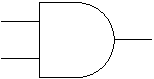
\includegraphics{../Introduction/ANDGate}
        \\AND gate
        \begin{tabular}{cc|c}
          \textbf{A} & \textbf{B} & \textbf{C} \\
          \hline
          0 & 0 & 0 \\
          0 & 1 & 0 \\
          1 & 0 & 0 \\
          1 & 1 & 1 \\
        \end{tabular}
      \end{center}
    \end{column}
    \begin{column}{3cm}
      \begin{center}
        \includegraphics{../Introduction/ORGate}
        \\OR gate
        \begin{tabular}{cc|c}
          \textbf{A} & \textbf{B} & \textbf{C} \\
          \hline
          0 & 0 & 0 \\
          0 & 1 & 1 \\
          1 & 0 & 1 \\
          1 & 1 & 1 \\
        \end{tabular}
      \end{center}
    \end{column}
    \begin{column}{3cm}
      \begin{center}
        \includegraphics{../Introduction/NOTGate}
        \\NOT gate (inverter)
        \begin{tabular}{c|c}
          \textbf{A} & \textbf{B} \\
          \hline
          0 & 1 \\
          1 & 0 \\
        \end{tabular}
      \end{center}
    \end{column}
  \end{columns}
\end{frame}

\begin{frame}{More logic gates}
  \begin{columns}
    \begin{column}{3cm}
      \begin{center}
        \includegraphics{NANDGate}
        \\NAND gate
        \begin{tabular}{cc|c}
          \textbf{A} & \textbf{B} & \textbf{C} \\
          \hline
          0 & 0 & 1 \\
          0 & 1 & 1 \\
          1 & 0 & 1 \\
          1 & 1 & 0 \\
        \end{tabular}
      \end{center}
    \end{column}
    \begin{column}{3cm}
      \begin{center}
        \includegraphics{NORGate}
        \\NOR gate
        \begin{tabular}{cc|c}
          \textbf{A} & \textbf{B} & \textbf{C} \\
          \hline
          0 & 0 & 1 \\
          0 & 1 & 0 \\
          1 & 0 & 0 \\
          1 & 1 & 0 \\
        \end{tabular}
      \end{center}
    \end{column}
  \end{columns}
\end{frame}

\subsection{Logic Families}

\begin{frame}{Logic families}
  There are two major logic families, or types of digital circuit chips.
  \begin{itemize}
    \item Transistor-transistor logic (TTL) circuits are built from bipolar junction transistors.
    \item Complementary metal-oxide semiconductor (CMOS) circuits are built from complementary MOSFET transistors.
  \end{itemize}
  We will explore both logic families.
\end{frame}

\section{CMOS Logic}

\begin{frame}{CMOS logic levels}
  Most CMOS circuits use a 5V power supply.  The logic levels are divided as follows.  Is this positive or negative logic?
  \begin{center}
    \includegraphics{CMOSLogicLevels}
  \end{center}
\end{frame}

\subsection{MOS Transistors}

\begin{frame}{What is a transistor?}
  \begin{block}{Concept}
    We can think of a transistor as a voltage controlled resistor or a voltage controlled switch.
  \end{block}
  \begin{columns}
    \begin{column}{3cm}
      \begin{center}
        \includegraphics{VoltageControlledResistor}
      \end{center}
    \end{column}
    \begin{column}{3cm}
      \begin{center}
        \includegraphics{VoltageControlledSwitch}
      \end{center}
    \end{column}
  \end{columns}
\end{frame}

\begin{frame}{NMOS transistor}
  \begin{columns}
    \begin{column}{3cm}
      \includegraphics{NMOSAnnotated}
    \end{column}
    \begin{column}{7cm}
      n-channel (NMOS) transistor
      \begin{itemize}
        \item The drain is normally at a higher voltage than the source.
        \item $V_{gs} = 0 \rightarrow$  high resistance (open).
        \item $V_{gs} \text{ positive} \rightarrow$ low high resistance (closed).
      \end{itemize}
    \end{column}
  \end{columns}
\end{frame}

\begin{frame}{PMOS transistor}
  \begin{columns}
    \begin{column}{3cm}
      \includegraphics{PMOSAnnotated}
    \end{column}
    \begin{column}{7cm}
      p-channel (PMOS) transistor
      \begin{itemize}
        \item The source is normally at a higher voltage than the drain.
        \item $V_{gs} = 0 \rightarrow$  high resistance (open).
        \item $V_{gs} \text{ negative} \rightarrow$ low high resistance (closed).
      \end{itemize}
    \end{column}
  \end{columns}
\end{frame}

\subsection{CMOS Logic Gates}

\begin{frame}{CMOS inverter}
  A CMOS inverter (or NOT gate) is made up of one NMOS and one CMOS transistor.
  \begin{center}
    \includegraphics{CMOSInverter}
  \end{center}
\end{frame}

\begin{frame}{CMOS inverter analysis}
  To analyze this circuit, use the following procedure:
  \begin{itemize}
    \item Create a table listing all of the possible input values, the state of each transistor, and the output value.
    \item For each input combination, determine the state of each transistor.
    \item Use the state of the transistors to determine the output value for each input combination.
  \end{itemize}
\end{frame}

This is called a function table:
\begin{tabular}{cccc}
  \textbf{$\textrm{V}_{\textrm{in}}$} & \textbf{Q1} & \textbf{Q2} & \textbf{$\textrm{V}_{\textrm{out}}$} \\
  \hline
  0V (LOW) & off & on & 5V (HIGH)\\
  5V (HIGH) & on & off & 0V (LOW)
\end{tabular}

\begin{frame}{Logical symbols for transistors}
  To help remember the behavior of NMOS and PMOS transistors, we will often use a logical representation of them.
  \vspace{0.5cm}
  \begin{columns}
    \begin{column}{5cm}
      \begin{center}
        \includegraphics{NMOSToNMOSLogical}
        \\
        NMOS transistor
      \end{center}
    \end{column}
    \begin{column}{5cm}
      \begin{center}
        \includegraphics{PMOSToPMOSLogical}
        \\
        PMOS transistor
      \end{center}
    \end{column}
  \end{columns}
\end{frame}

\begin{frame}{CMOS NAND Gate}
  \begin{center}
    \includegraphics[scale=0.8]{CMOSNANDGate}
  \end{center}
\end{frame}

\begin{tabular}{ccccccc}
  \textbf{A} & \textbf{B} & \textbf{Q1} & \textbf{Q2} & \textbf{Q3} & \textbf{Q4} & \textbf{Z} \\
  \hline
  L & L & off & on & off & on & H\\
  L & H & off & on & on & off & H\\
  H & L & on & off & off & on & H\\
  H & H & on & off & on & off & L\\
\end{tabular}

\begin{frame}{CMOS NOR Gate}
  \begin{center}
    \includegraphics[scale=0.8]{CMOSNORGate}
  \end{center}
\end{frame}

\begin{tabular}{ccccccc}
  \textbf{A} & \textbf{B} & \textbf{Q1} & \textbf{Q2} & \textbf{Q3} & \textbf{Q4} & \textbf{Z} \\
  \hline
  L & L & off & on & on & on & H\\
  L & H & off & on & on & off & L\\
  H & L & off & off & off & on & L\\
  H & H & on & off & on & off & L\\
\end{tabular}

\section{CMOS Static Electric Behavior}

\begin{frame}{Blue pill or red pill?}
  \begin{block}{Digital Abstraction}
    Generally, we assume that digital circuits operate on digital inputs to produce digital outputs.  However, this is an abstraction of the analog truth.
  \end{block}
  \begin{itemize}
    \item CMOS circuits behave perfectly on paper, but in the real world they are subject to constraints.
    \item Manufacturers publish these constraints in product data sheets.
    \item When building real circuits, it is important to be familiar with product data sheets.
  \end{itemize}
\end{frame}

\subsection{Logic Levels}

\begin{frame}{More on logic levels}
  \begin{columns}
    \begin{column}{4cm}
      \includegraphics[scale=0.6]{CMOSLogicLevelsDetailed}
    \end{column}
    \begin{column}{6cm}
      Output specifications
      \begin{itemize}
        \item $\textrm{V}_{\textrm{OHmin}} = \textrm{V}_{\textrm{CC}} - 0.1$ is the minimum output voltage in the HIGH state
        \item $\textrm{V}_{\textrm{OLmax}} = \textrm{V}_{\textrm{CC}} + 0.1$ is the maximum output voltage in the LOW state
      \end{itemize}
      Input specifications
      \begin{itemize}
        \item $\textrm{V}_{\textrm{IHmin}} = 0.7 \cdot \textrm{V}_{\textrm{CC}}$ is the minimum HIGH input voltage
        \item $\textrm{V}_{\textrm{ILmax}} = 0.3 \cdot \textrm{V}_{\textrm{CC}}$ is the maximum LOW input voltage
      \end{itemize}
    \end{column}
  \end{columns}
\end{frame}

\begin{frame}{DC noise margin}
  \begin{definition}
    The \alert{DC noise margin} is a measure of how much noise is required to corrupt an output voltage so that it cannot be correctly recognized as an input voltage.
  \end{definition}
  \begin{columns}
    \begin{column}{4cm}
      \includegraphics[scale=0.6]{CMOSLogicLevelsDetailedWithNoiseMargin}
    \end{column}
    \begin{column}{6cm}
      \begin{itemize}
        \item HIGH state: $\textrm{V}_{\textrm{OHmin}} - \textrm{V}_{\textrm{IHmin}}$
        \item LOW state: $\textrm{V}_{\textrm{ILmax}} - \textrm{V}_{\textrm{OLmax}}$
      \end{itemize}
    \end{column}
  \end{columns}
\end{frame}

\subsection{Loading CMOS Devices}

\begin{frame}{Resistive loads}
  \begin{itemize}
    \item Many loads can be modeled by a Th\'evenin equivalent circuit.
    \item A MOSFET transistor in the "on" state has a non-zero resistance.
    \item A MOSFET transistor in the "off" state has a non-infinite resistance.
  \end {itemize}
\end{frame}

\begin{frame}{Effect of resistive loads on a CMOS inverter}
  \begin{center}
    \includegraphics[scale=0.8]{ResistiveLoadsGraph}
  \end{center}
\end{frame}

\begin{frame}{Loading and fanout}
  \begin{definition}
    The \alert{fanout} of a gate is the number of inputs (e.g. other gates) it can drive.
  \end{definition}
  Overloading a CMOS gate can cause problems.
  \begin{itemize}
    \item Reduce the DC noise margin
    \item Increase the operating temperature
  \end{itemize}
\end{frame}

Both problems can be very insidious, because they may never show up in the lab, so the manufacturer's specifications should always be followed.

\subsection{Rules of Thumb}

\begin{frame}{CMOS static electric behavior rules of thumb}
  \begin{itemize}
    \item Be familiar it the data sheets for all ICs in your circuit.
    \item Know the DC noise margins and stay well within them.
    \item Do not overload your devices.
    \item Never leave inputs floating.
    \item Watch out for static electricity.
  \end{itemize}
\end{frame}

\section{CMOS Dynamic Electric Behavior}

\subsection{Transition Time}

\begin{frame}{Transition time}
  Transitions between logic levels are not instantaneous.
  \begin{block}{Rise Time}
    \alert{Rise time} measures the time for a circuit to transition from LOW to HIGH.
  \end{block}
  \begin{block}{Fall Time}
    \alert{Fall time} measures the time for a circuit to transition from HIGH to LOW.
  \end{block}
  To minimize transition time, minimize the capacitance of outputs by controlling fanout and load.
\end{frame}

\subsection{Propagation Delay}

\begin{frame}{Propagation delay}
  \begin{definition}
    The \alert{propagation delay} of a circuit is the amount of time required for an input to produce a output.
  \end{definition}
  \begin{itemize}
    \item In general the more complex a circuit, the longer the propagation delay.
    \item Different outputs from a circuit may have different propagation delays.
  \end{itemize}
\end{frame}

\subsection{Power Consumption}

\begin{frame}{Power consumption}
  One advantage of CMOS circuits over other types of digital logic is their low power requirements.
  \begin{itemize}
    \item Holding and input value requires very little power.
    \item And input transition may require significant power for a short period of time.
  \end{itemize}
  Therefore, the number of transitions should be minimized in order to minimize power requirements.
\end{frame}

\section{Digital Circuit Design}

\begin{frame}{Circuit design process}
  \begin{block}{Design Procedure}
    \begin{enumerate}
      \item Write the truth table for the circuit.
      \item Start with a known circuit(logic symbols) and truth table, and augment it to produce the desired truth table.
      \item Convert the logic symbols to the desired type of transistors.
    \end{enumerate}
  \end{block}
\end{frame}

\begin{frame}{The exclusive OR gate (XOR)}
  \begin{block}{Problem}
    Design a two input digital circuit such that the output of the circuit is HIGH if the inputs differ, and LOW if the inputs are the same.
  \end{block}
\end{frame}

\begin{itemize}
  \item This looks similar to an OR gate.
  \item Think about doing a logic operation on the result of two truth tables (in this case, OR and NAND).
\end{itemize}

\begin{frame}{Solution}
  \begin{columns}
    \begin{column}{4cm}
      Truth table:\\
      \begin{center}
        \begin{tabular}{cc|c}
          \textbf{A} & \textbf{B} & \textbf{Z} \\
          \hline
          0 & 0 & 0 \\
          0 & 1 & 1 \\
          1 & 0 & 1 \\
          1 & 1 & 0 \\
        \end{tabular}
      \end{center}
    \end{column}
    \begin{column}{6cm}
      Logic diagram:\\
      \begin{center}
        \includegraphics{XORLogicCircuit}
      \end{center}
    \end{column}
  \end{columns}
  \medskip
  Conversion to a transistor circuit is left as an exercise.
\end{frame}
\end{document}
